%%%%%%%%%%%%%%%%%%%%%%%%%%%%%%%%%%%%%%%%%%%%%%%%%%%%%%%%%%%%%%%%%%%%%%%%
%
% V2D Challenge Track 3 -- Technical Report (2-Page Main Text + Appendix)
% Build: pdflatex main && bibtex main && pdflatex main && pdflatex main
%
%%%%%%%%%%%%%%%%%%%%%%%%%%%%%%%%%%%%%%%%%%%%%%%%%%%%%%%%%%%%%%%%%%%%%%%%

\pdfoutput=1

\documentclass[10pt]{nvidiaextabstract}

\usepackage{microtype}
\usepackage{multirow}
\usepackage{subcaption}
\usepackage{xspace}
\usepackage{booktabs}
\usepackage{tikz}
\usetikzlibrary{shapes.geometric, arrows.meta, positioning}

\newcommand{\todo}[1]{\textcolor{red}{[TODO: #1]}}
\newcommand{\ownauc}{\ensuremath{\mathrm{AUC}_{\text{own}}}\xspace}

\venue{From Human Videos to Dexterous Robot Capability (CoRL 2026)}

\submissionID{\todo{Gravity Aligned}}

\title{Fix the Reference, Not the Policy: Egocentric Video to Dexterous Robot Rollouts}
\subtitle{V2D Challenge Track 3 Technical Report}
\shorttitle{Fix the Reference, Not the Policy}

\author[1*]{Edmond Wang}
\author[1*]{Haisen Kang}
\author[1*]{Wentao Cao}
\author[1*]{James Zhao}
\author[1]{\todo{Add remaining authors or remove}}
\affil[1]{Carnegie Mellon University}
\affil[ ]{\texttt{\{edmondwa, haisenk, wentaoc, jameszh2\}@andrew.cmu.edu}}
\correspondingauthor{edmondwa@andrew.cmu.edu}

\begin{abstract}
\textbf{Abstract:}
We convert single egocentric videos into simulated rollouts of a bimanual Sharpa robot-hand tracking policy for Track~3 of the NVIDIA Isaac Video-to-Data (V2D) Challenge. Starting from the V2D baseline, we replace monocular depth with calibrated metric stereo depth, upgrade segmentation to SAM~3, select object meshes across keyframes, repair physically implausible references, and train per-episode FlashSAC policies. Across more than 440 training runs, \emph{physical defects in the kinematic reference, rather than the RL recipe, bottleneck tracking on hard episodes}: repairs improved individual episodes by up to $+0.50$ own-reference AUC, whereas global reward or exploration changes hurt on average. Combining three reconstruction streams via a ground-truth-free selection rule achieves \textbf{0.780 ADD-AUC} (0.95 SP-SR, 0.65 MP-SR) on the hidden leaderboard, up from 0.295 for a static baseline.
\end{abstract}

\definecolor{NvidiaGreen}{RGB}{118, 185, 0}

\begin{document}

\maketitle

%%%%%%%%%%%%%%%%%%%%%%%%%%%%%%%%%%%%%%%%%%%%%%%%%%%%%%%%%%%%%%%%%%%%%%%%
\section{Introduction}
\label{sec:intro}

Egocentric human video is the most scalable source of manipulation demonstrations, yet transferring it to a simulated dexterous robot remains brittle. Track~3 of the NVIDIA V2D Challenge~\cite{v2d,v2ddata} evaluates this full pipeline on 20 scored clips (36 object instances): submissions provide reconstructed object meshes and 6-DoF trajectories generated by \emph{executing a learned robot policy in simulation}, scored against hidden motion capture.

Errors compound across (i)~metric scale and placement in reconstruction, (ii)~physically impossible references (mid-air releases, 25\,cm hand--object gaps, $40^\circ$/frame unobservable spin) and (iii)~policy tracking under contact. On public data the stock monocular baseline (0.292 ADD-AUC) scores below holding objects still at frame~0 (0.309). Our central finding is that eliminating physical defects in the kinematic reference is far more effective than tuning the RL policy. Full text for every section is in Appendix~\ref{sec:appendix}.

\begin{figure*}[t]
  \centering
  \resizebox{\textwidth}{!}{%
  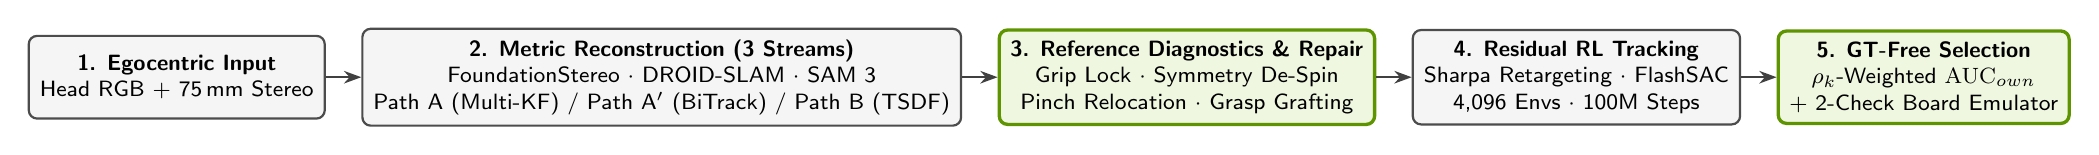
\begin{tikzpicture}[
    node distance=0.45cm,
    box/.style={rectangle, rounded corners=3pt, draw=black!70, fill=gray!8, thick, minimum height=1.05cm, align=center, font=\footnotesize\sffamily, inner sep=4pt},
    greenbox/.style={rectangle, rounded corners=3pt, draw=NvidiaGreen!80!black, fill=NvidiaGreen!12, very thick, minimum height=1.05cm, align=center, font=\footnotesize\sffamily, inner sep=4pt},
    arrow/.style={-{Stealth[length=2.2mm, width=1.6mm]}, thick, draw=black!75}
  ]
    \node[box] (video) {\textbf{1. Egocentric Input}\\Head RGB + 75\,mm Stereo};
    \node[box, right=of video] (recon) {\textbf{2. Metric Reconstruction (3 Streams)}\\FoundationStereo $\cdot$ DROID-SLAM $\cdot$ SAM~3\\Path A (Multi-KF) / Path A$'$ (BiTrack) / Path B (TSDF)};
    \node[greenbox, right=of recon] (repair) {\textbf{3. Reference Diagnostics \& Repair}\\Grip Lock $\cdot$ Symmetry De-Spin\\Pinch Relocation $\cdot$ Grasp Grafting};
    \node[box, right=of repair] (policy) {\textbf{4. Residual RL Tracking}\\Sharpa Retargeting $\cdot$ FlashSAC\\4,096 Envs $\cdot$ 100M Steps};
    \node[greenbox, right=of policy] (select) {\textbf{5. GT-Free Selection}\\$\rho_k$-Weighted $\ownauc$\\+ 2-Check Board Emulator};

    \draw[arrow] (video) -- (recon);
    \draw[arrow] (recon) -- (repair);
    \draw[arrow] (repair) -- (policy);
    \draw[arrow] (policy) -- (select);
  \end{tikzpicture}%
  }
  \vspace{-4mm}
  \caption{Overview of our Track~3 pipeline: metric reconstruction, reference repair, per-episode policy training and ground-truth-free selection.}
  \label{fig:overview}
  \vspace{-3mm}
\end{figure*}

%%%%%%%%%%%%%%%%%%%%%%%%%%%%%%%%%%%%%%%%%%%%%%%%%%%%%%%%%%%%%%%%%%%%%%%%
\section{Approach}
\label{sec:approach}

Figure~\ref{fig:overview} illustrates our five-stage architecture built atop \texttt{video\_to\_data} (commit \texttt{8c778f9})~\cite{v2d}.

%----------------------------------------------------------------------
\subsection{Metric-Stereo 3D Reconstruction}
\label{sec:recon}

The stock baseline's monocular MoGe-2~\cite{wang2025moge2} depth inflated world scale by a median $1.33\times$ over 69 audited reconstructions, and its Gaussian-splatting refinement~\cite{kerbl20233dgs} diverged. We replace this front-end with three complementary metric streams (Appendix~\ref{app:detail-recon}).

\textbf{Path A (Multi-Keyframe Metric Stereo).} FoundationStereo~\cite{wen2025foundationstereo} depth on the 75\,mm stereo pair ($1.3$--$1.9\%$ error against SGBM, vs.\ $14$--$18\%$ for rescaled MoGe-2) anchors DROID-SLAM~\cite{teed2021droid} and FoundationPose~\cite{wen2024foundationpose}. SAM~3~\cite{carion2025sam3} raises mask IoU from 0.786 to 0.912 (ep41), selecting among 12 SAM~3D~\cite{sam3dteam2025sam3d} candidates lifts 11-episode public AUC from 0.514 to 0.649, and a CoTracker3~\cite{karaev2025cotracker3} referee resolves $180^\circ$ flips (ep18: $0.755 \rightarrow 0.916$).

\textbf{Path A$'$ (Fixed-Mesh Bidirectional Tracking).} Path~A$'$ masks dynamic hands and objects out of DROID-SLAM, fits one uniform metric scale per SAM~3D mesh over three support frames via Pareto selection, and runs \emph{bidirectional} FoundationPose from a verified anchor frame without scale sweeps or EKF drift. On public ep27 this reduced inter-object RPE from 41.4 to 1.6\,cm (AUC $0.267 \rightarrow 0.913$); the retained reconstruction reaches 0.908 playback ADD-AUC over all 20 public episodes. Inertial origins, frame-0 seating and per-frame hold gates are repaired as scene hygiene (Appendix~\ref{app:patha-prime}).

\textbf{Path B (Contact-Segmented Kinematic Inversion).} Without generative priors, Path~B fuses multi-clip stereo depth into one canonical mesh per object via TSDF pooling~\cite{curless1996volumetric,zhou2018open3d} and, during grasps, inverts object pose from the carrying wrist with one rigid offset per grasp and a bounded per-frame correction inspired by ROHIT~\cite{rohit}, reaching 0.829 playback AUC on the public episodes.

%----------------------------------------------------------------------
\subsection{Physics-Consistent Reference Diagnostics and Repair}
\label{sec:repair}

Retargeted references frequently violate physics. Pre-training detectors flag ghost motion, contact and grasp gaps, and rotational tremor; flagged episodes receive targeted, ground-truth-free repairs (Appendix~\ref{app:detail-repair}): \emph{grip locking} when hands open in mid-air (ep14: 0.58 to 0.85 \ownauc); \emph{symmetry-aware de-spinning} of cup twist that ADD ignores but the $0.5$\,rad termination does not (ep8: 0.917); \emph{pinch relocation and hand refill} (ep3: $0.37 \rightarrow 0.871$; ep20: $0.38 \rightarrow 0.838$); \emph{cross-stream grasp grafting} of Path~A contacts onto Path~A$'$ objects (ep16: 0.931); and \emph{assembly repairs} for slot insertion (ep25: $0.546 \rightarrow 0.827$).

%----------------------------------------------------------------------
\subsection{Residual RL Tracking and GT-Free Selection}
\label{sec:policy}

We train one FlashSAC~\cite{flashchord,haarnoja2018sac} policy per episode (4,096 parallel environments, 100M steps, $\sim$45\,min on one L40S), evaluate checkpoints every 5M steps from 70M, and retain the best rollout, since the final checkpoint is suboptimal in $71\%$ of runs (Appendix~\ref{app:detail-policy}).

Because a policy that perfectly tracks a misplaced reconstruction scores $\ownauc \approx 1.0$ yet poorly on the leaderboard, we select per episode $c^\star_e = \arg\max_{c} \rho_{k(c)} \cdot \ownauc(c)$, where $\rho_k = \mathrm{AUC}_{\text{Kaggle}} / \overline{\ownauc}$ is a stream's aggregate transfer ratio ($\rho_{\text{A}} = 0.81$, $\rho_{\text{A}'} = 0.86$). Final single-episode refinements must also pass a \emph{two-check gate}: a local board emulator and a rendered camera-space proxy (Spearman $r=0.956$ and $0.912$ with true leaderboard deltas across 14 swaps).

%%%%%%%%%%%%%%%%%%%%%%%%%%%%%%%%%%%%%%%%%%%%%%%%%%%%%%%%%%%%%%%%%%%%%%%%
\section{Experiments and Results}
\label{sec:experiments}

\begin{table}[!t]
  \centering\footnotesize
  \setlength{\tabcolsep}{2pt}
  \resizebox{\columnwidth}{!}{%
  \begin{tabular}{@{}lccccccc@{}}
    \toprule
    \textbf{Milestone} & \textbf{\ownauc} & \textbf{AUC}$\uparrow$ & \textbf{SP}$\uparrow$ & \textbf{MP}$\uparrow$ & \textbf{RPE}$\downarrow$ & \textbf{MPPE}$\downarrow$ & \textbf{CD-O}$\downarrow$ \\
    \midrule
    Static frame-0 baseline & -- & 0.295 & 0.25 & 0.00 & 19.78 & 14.87 & 0.473 \\
    GT-free ensemble (A + A$'$) & 0.895 & 0.752 & 0.90 & 0.45 & 4.35 & 3.61 & 0.410 \\
    \textbf{Team final} & \textbf{0.912} & \textbf{0.780} & \textbf{0.95} & \textbf{0.65} & \textbf{3.87} & \textbf{3.28} & \textbf{0.322} \\
    \bottomrule
  \end{tabular}}
  \vspace{-2mm}
  \caption{Leaderboard milestones (errors in cm; full history in Table~\ref{tab:kaggle}).}
  \label{tab:headline}
  \vspace{-3mm}
\end{table}

\textbf{Repair beats recipe.} Across 440+ runs ($\sim$850 GPU-hours; Appendix Table~\ref{tab:ablations}), every targeted reference repair succeeded, lifting episodes by $+0.07$ to $+0.50$ \ownauc. Global changes did not: WIDE exploration beat LOOSE on 7 of 19 scenes but lost $0.03$ AUC on average, and smaller keypoint kernels or force-closure rewards degraded tracking. Stricter termination helped specific episodes (ep33: $0.637 \rightarrow 0.827$). Open-loop replay scores only $0.11$--$0.30$, so closed-loop residual RL is essential.

\textbf{Leaderboard.} Path~A tracked better than Path~A$'$ (mean \ownauc $0.888$ vs.\ $0.741$) through tighter contacts, but Path~A$'$ transferred better ($\rho$ 0.86 vs.\ 0.81) through better multi-object placement; per-episode selection lifted our score from 0.711 to 0.752 (Appendix Table~\ref{tab:kaggle}). Four single-episode hand-repair rollouts reached 0.765 (Appendix Table~\ref{tab:provenance}), and further swaps and best-of-$N$ rollout re-draws on the same base brought the team to \textbf{0.780 ADD-AUC}, \textbf{0.95 SP-SR}, \textbf{0.65 MP-SR}, 3.87\,cm RPE, 3.28\,cm MPPE and \textbf{0.322\,cm CD-O} at the close (rank sum 81). Remaining errors stem from convex hulls preventing cup nesting (ep10), PD wrist lag knocking thin tools aside, and $180^\circ$ ambiguities on symmetric boards.

%%%%%%%%%%%%%%%%%%%%%%%%%%%%%%%%%%%%%%%%%%%%%%%%%%%%%%%%%%%%%%%%%%%%%%%%
\section{Industry Relevance}
\label{sec:industry}

\textbf{Economic Viability.} Commodity stereo-headset video becomes physically valid dexterous rollouts with no motion capture, gloves or teleoperation, at $\sim$2.5 GPU-hours ($\approx\$3.00$ at spot rates) per demonstration.
\textbf{Data Flywheel.} Automated detectors triage incoming video without ground truth, and rollout failures pinpoint upstream perception defects.
\textbf{Complexity Reduction.} Stereo depth eliminates monocular scale recovery and pose scale sweeps; repaired references let a closed-form selection rule replace per-episode reward engineering (Appendix~\ref{app:detail-industry}).

\textbf{Innovation.} We optimize the physical validity of the reference rather than the RL policy, through symmetry-aware de-spinning, grip locking, cross-stream grafting, contact-segmented wrist inversion and transfer-calibrated GT-free selection.

%%%%%%%%%%%%%%%%%%%%%%%%%%%%%%%%%%%%%%%%%%%%%%%%%%%%%%%%%%%%%%%%%%%%%%%%
\section{Conclusion}
\label{sec:conclusion}

Shifting optimization from the RL policy to the physical validity of the kinematic reference raised Track~3 performance from a 0.295 baseline to 0.780 ADD-AUC. Future work will close the loop from rollouts back to differentiable reconstruction and train one multi-task policy.

%%%%%%%%%%%%%%%%%%%%%%%%%%%%%%%%%%%%%%%%%%%%%%%%%%%%%%%%%%%%%%%%%%%%%%%%
% Acknowledgments, references and appendices do not count against the 2-page
% main-text limit (nvidiaextabstract.cls), which is checked where they begin.
%%%%%%%%%%%%%%%%%%%%%%%%%%%%%%%%%%%%%%%%%%%%%%%%%%%%%%%%%%%%%%%%%%%%%%%%
\begin{acks}
Compute was provided by the CMU Babel cluster. CoTracker3 is used under CC-BY-NC.
\end{acks}

\bibliographystyle{plainnat}
\bibliography{references}

%%%%%%%%%%%%%%%%%%%%%%%%%%%%%%%%%%%%%%%%%%%%%%%%%%%%%%%%%%%%%%%%%%%%%%%%
\appendix

\section{Supplementary Material and Detailed Logs}
\label{sec:appendix}

\subsection{Compliance and Code}
\label{sec:compliance}
\textbf{Challenge Rule Compliance.} Every submitted trajectory is a recorded rollout of a trained FlashSAC policy executed inside the official FlashCHORD evaluator (revision \texttt{8c778f90}); no kinematic reconstructions or reference trajectories are submitted. All 36 object meshes are reconstructed strictly from the challenge RGB/stereo videos; no public ground-truth 3D scans were used for mesh generation, registration, or scoring. Because parallel physics evaluation exhibits run-to-run variance (Appendix Table~\ref{tab:rescore}), promising checkpoints are evaluated across $N=4$ rollouts and the highest-scoring recorded rollout against its own reference is retained.

\textbf{Code \& Container Provenance.} The code that produced the submissions is in our repository (\href{https://github.com/zjifan121-source/NVIDIA_V2D_Egocentric}{\texttt{github.com/\allowbreak zjifan121-source/\allowbreak NVIDIA\_V2D\_Egocentric}}) at commit \texttt{de66fea3ae7c99ba96458f3cd9d1b77f5f94b4ff} (training pipeline, campaign tooling and hand-fix tools), with the Path~A$'$ scene-hygiene tools in PR~\#24; every submitted row carries the kit's provenance hashes (commit URL, evaluation script and code, packer, uploader, policy checkpoint), listed for the six-board base file (sha256 \texttt{c8fcd7df\ldots}, Kaggle 57978563) in Appendix~\ref{app:provenance}. A reproduction container will be provided after 12 November, as the challenge requires. Reconstructed scenes, checkpoints and rollouts are archived at \texttt{huggingface.co/\allowbreak datasets/\allowbreak rose-tea-cafe/\allowbreak v2d-t3-recon}.

\subsection{Extended Introduction and Contributions}
\label{app:detail-intro}
\textbf{Full Abstract.} Transforming unconstrained egocentric human manipulation videos into physically valid dexterous robot trajectories requires both accurate 3D perception and robust control. In Track~3 of the NVIDIA Isaac Video-to-Data (V2D) Challenge, we convert single egocentric videos into simulated rollouts of a bimanual Sharpa robot-hand tracking policy. Starting from the V2D baseline, we replace monocular depth with calibrated metric stereo depth, upgrade segmentation to SAM~3, select object meshes across multi-view keyframes, enforce physics-consistent reference repairs, and train per-episode FlashSAC tracking policies. Across more than 440 policy training runs, we find a clear governing principle: \emph{physical defects in the kinematic reference, rather than the RL optimization recipe, bottleneck policy tracking on hard episodes}. Repairing implausible reference grasps and spin noise improved individual episode tracking by up to $+0.50$ own-reference AUC, whereas global changes to reward shaping or exploration hurt average performance. Combining three complementary reconstruction streams via a ground-truth-free selection rule achieves \textbf{0.780 ADD-AUC} (0.95 SP-SR, 0.65 MP-SR) on the hidden Track~3 leaderboard, up from 0.295 for a static baseline.

\textbf{Full Figure~\ref{fig:overview} Caption.} Overview of our Track~3 pipeline. Calibrated stereo depth and three complementary reconstruction streams produce metric 3D scenes. Physics-consistent reference repairs resolve contact and spin defects prior to training per-episode FlashSAC policies in FlashCHORD, followed by ground-truth-free candidate selection.

Egocentric human video is the most scalable source of manipulation demonstrations, yet bridging the embodiment and physics gap to a simulated dexterous robot remains brittle. Track~3 of the NVIDIA V2D Challenge~\cite{v2d,v2ddata} evaluates this full pipeline across 20 scored egocentric video clips (36 object instances; 16 two-object scenes). Submissions must output reconstructed 3D object meshes (without using public ground-truth scans) and 6-DoF object trajectories generated strictly by \emph{executing a learned robot policy rollout in simulation}. Rollouts are scored against hidden motion-capture ground truth primarily via ADD-AUC (1--9\,cm thresholds), alongside single/multi-pose success rates (SP-SR, MP-SR), relative/mean pose errors (RPE, MPPE), and mesh Chamfer distance (CD-O).

Errors compound across three stages: (i)~metric scale and relative placement errors during 3D reconstruction (exacerbated by single-anchor frame-0 evaluation alignment in multi-object scenes); (ii)~physically impossible reference trajectories (e.g., mid-air object releases, 25\,cm hand--object contact gaps, or unobservable $40^\circ$/frame axial spin noise); and (iii)~policy tracking failure under contact-rich dynamics. An oracle decomposition on the 20 public development episodes (Appendix, Table~\ref{tab:oracle}) revealed that baseline monocular playback (0.292 ADD-AUC) performs worse than holding objects stationary at frame~0 (0.309), driven primarily by a $1.33\times$ monocular scale inflation. Furthermore, while FlashSAC policies achieve $0.90+$ AUC when tracking clean ground-truth references, they suffer a severe ``policy tax'' on raw reconstructed trajectories. Our central finding is that eliminating physical defects in the kinematic reference is far more effective than tuning the RL policy.

\textbf{Contributions:}
\begin{itemize}\setlength{\itemsep}{1pt}\setlength{\parskip}{0pt}
  \item \textbf{Metric-Stereo Reconstruction:} Replacing monocular MoGe-2 depth with calibrated FoundationStereo depth, upgrading to SAM~3 segmentation, selecting multi-keyframe meshes with cross-episode video pooling, and removing destructive Gaussian splatting refinement.
  \item \textbf{Physics-Consistent Reference Repairs:} Automated, ground-truth-free kinematics repairs—including grip locking, symmetry-aware de-spinning, pinch relocation, and grasp grafting—paired with pre-training defect detectors.
  \item \textbf{Large-Scale Policy Study:} An empirical analysis of 440+ FlashSAC runs demonstrating that targeted scene repair consistently outperforms global reward and exploration tuning.
  \item \textbf{Ground-Truth-Free Ensemble Selection:} Combining three distinct reconstruction paradigms via leaderboard-calibrated transfer ratios and a local board emulator, lifting hidden leaderboard performance from 0.295 to \textbf{0.780 ADD-AUC}.
\end{itemize}

\subsection{Extended Method Details}
\label{app:detail-method}

\subsubsection{Reconstruction}
\label{app:detail-recon}
The stock baseline estimates depth monocularly via MoGe-2~\cite{wang2025moge2}, segments objects with Grounding~DINO~\cite{liu2024groundingdino} + SAM~2.1~\cite{ravi2025sam2}, generates single-view meshes with SAM~3D Objects~\cite{sam3dteam2025sam3d}, tracks poses via FoundationPose~\cite{wen2024foundationpose} over a 36-scale sweep, reconstructs MANO hands~\cite{romero2017mano} with WiLoR~\cite{potamias2025wilor}/HaMeR~\cite{pavlakos2024hamer}, and jointly refines camera and object tracks via 3D Gaussian splatting~\cite{kerbl20233dgs,ye2025gsplat}. Auditing 69 baseline reconstructions revealed severe failures: MoGe-2 inflated world scale by a median of $1.33\times$ (range $1.09$--$1.70\times$), text prompts occasionally segmented the entire tabletop ($11.8\times$ mesh inflation), and Gaussian splatting refinement frequently diverged (turning 0.17\,m of camera motion into 14.7\,m on ep13).

We replace this brittle front-end with a shared metric foundation across three complementary reconstruction streams:

\textbf{Path A (Multi-Keyframe Metric Stereo).} We rectify the headset's factory-calibrated 75\,mm monochrome stereo pair, remove residual 1--2\,px row offsets via ORB matching, and compute dense metric depth using FoundationStereo~\cite{wen2025foundationstereo} (cross-checked against SGBM~\cite{hirschmuller2008sgm} to within $1.3$--$1.9\%$ median error, vs.\ $14$--$18\%$ for per-frame rescaled MoGe-2). Stereo depth directly anchors DROID-SLAM~\cite{teed2021droid} and FoundationPose. We upgrade object segmentation to text-prompted SAM~3~\cite{carion2025sam3} with bidirectional propagation and adaptive confidence fallback ($0.3 \rightarrow 0.15$), raising mask IoU from 0.786 to 0.912 (ep41). We also detect late-entering hands missed at frame~0 (occurring in 6 of 20 scored clips) via MediaPipe~\cite{zhang2020mediapipehands} and correct a hard-coded 30\,fps loader bug that time-compressed 20.254\,fps videos by $1.48\times$. To combat single-view mesh inflation, we sample 12 SAM~3D candidates (6 unoccluded keyframes $\times$ 2 seeds), select the mesh minimizing occlusion-aware silhouette IoU and stereo depth residuals across 40 frames (lifting 11-episode public AUC from 0.514 to 0.649), and fit 3-axis per-object scales (reducing CD-O from 0.584 to 0.476\,cm). We also employ \emph{cross-episode video mesh pooling} (reconstructing an object from its clearest video clip and reusing that reconstructed mesh across episodes, using zero ground-truth scans). Finally, we disable Gaussian splatting refinement ($+0.114$ AUC on practice clips) and add a CoTracker3~\cite{karaev2025cotracker3} 64-point optical flow referee to resolve $180^\circ$ symmetry flips (lifting ep18 from 0.755 to 0.916).

\textbf{Path A$'$ (Fixed-Mesh Bidirectional Tracking).} To maximize inter-object geometric consistency, Path~A$'$ masks dynamic hands and objects out of DROID-SLAM, fits a single uniform metric scale per SAM~3D mesh across three support frames via Pareto selection (IoU, depth residual, coverage), and runs \emph{bidirectional} FoundationPose from a verified anchor frame without scale sweeps or EKF drift. Optional silhouette/depth-constrained mesh deformation and stereo landmark stabilization are logged as separate candidate bundles. On public ep27 this reduced inter-object RPE from 41.4 to 1.6\,cm (AUC $0.267 \rightarrow 0.913$); the retained reconstruction reaches 0.908 playback ADD-AUC over all 20 public episodes. We further enforce simulation scene hygiene (Appendix~\ref{app:patha-prime}): shifting URDF inertial origins to shell centroids, seating frame-0 objects onto the support plane within $2$\,mm, and enforcing per-frame contact hold gates.

\textbf{Path B (Contact-Segmented Kinematic Inversion).} Operating without generative 3D priors, Path~B fuses multi-clip stereo depth into one canonical mesh per object via gated Open3D TSDF pooling~\cite{curless1996volumetric,zhou2018open3d}, symmetry completion, and screened Poisson reconstruction~\cite{kazhdan2013screened} with CoACD~\cite{wei2022coacd} collision hulls. Frames are segmented into \emph{static}, \emph{grasp}, or \emph{unstable}; a rest ends only at hand contact, and each hand is assigned to one object at a time. Static segments are solved by multi-start ICP with upright and stacking priors, the frame-0 anchor pose is fitted jointly over all pre-contact frames (it fixes the scorer's scene alignment), and rests are settled in MuJoCo~\cite{todorov2012mujoco}. During grasps the pose is inverted from the carrying wrist, $T_{\text{obj}}(t) = T_{\text{wrist}}(t)\,T\,D(t)$, with one rigid wrist-to-object offset $T$ per grasp and a bounded per-frame correction $D(t)$ ($\le 5$\,mm, $3^\circ$/frame) on a depth--silhouette residual, inspired by ROHIT~\cite{rohit}; lost grasps and unseen-wrist gaps are bridged by wrist-carried or frame-to-frame followed tracks. A gated FoundationPose refiner~\cite{wen2024foundationpose} then polishes moving frames, keeping a refined pose only where its own score and the mask IoU do not worsen. Path~B reaches 0.829 playback AUC across the 20 public episodes.

\subsubsection{Reference Diagnostics and Repair}
\label{app:detail-repair}
Retargeting reconstructed MANO hands to simulated Sharpa hands frequently yields references that violate physics. Baseline loader leveling and hand attachment help (lifting public ep41 own-reference tracking from 0.324 to 0.743), but hard episodes fail unless specific physical defects are repaired. Before training, our automated detectors scan references for \emph{ghost motion} ($>0.25$\,cm or $>3^\circ$/frame without a hand within $r+3$\,cm), \emph{contact gaps} (lifted $>2$\,cm with zero reference contacts), \emph{grasp gaps} (median fingertip-to-surface distance $>4$\,cm during lifts), and \emph{rotational tremor} ($>3^\circ/\text{frame}^2$). Flagged episodes undergo targeted, ground-truth-free repairs:
\begin{itemize}\setlength{\itemsep}{1pt}\setlength{\parskip}{0pt}
  \item \textbf{Grip Locking (\texttt{hold\_hand}):} When reconstructed hands prematurely open in mid-air while the object descends (e.g., ep14 frame 81, 9\,cm above the table), contact rewards penalize the policy for holding on. Locking the object-relative grip with 4-frame SLERP blending boosts fresh training seeds from 0.58 to 0.85 \ownauc.
  \item \textbf{Symmetry-Aware De-Spinning (\texttt{despin}):} FoundationPose tracks on cylindrical cups exhibit unobservable axial twist spikes of $21$--$43^\circ$/frame. While the ADD metric is invariant to symmetric twist, the policy's $0.5$\,rad orientation termination is not. Projecting out axial twist via swing decomposition, $R'_t = \mathrm{swing}(a_0 \rightarrow a_t)R_0$, and Gaussian smoothing ($\sigma=2$) lifts ep8 to 0.917 \ownauc.
  \item \textbf{Pinch Relocation \& Hand Refill:} When a lifting hand is reconstructed $24$--$28$\,cm away from the object (ep3) or drifts off-screen (ep20), we translate the wrist by a constant object-local offset to place the thumb--index midpoint on the rim, or refill off-screen hand trajectories in the object frame (ep3: $0.37 \rightarrow 0.871$; ep20: $0.38 \rightarrow 0.838$).
  \item \textbf{Cross-Stream Grasp Grafting (\texttt{graft\_grasps}):} Because Path~A excels at hand--object contact while Path~A$'$ excels at object placement, we graft Path~A's object-relative wrist and finger trajectories onto Path~A$'$ object tracks during active grasps (closing ep16's grasp gap from 8.62 to 1.96\,cm and reaching 0.931 \ownauc).
  \item \textbf{High-Precision Assembly:} For tight two-board slot insertion (ep25), combining pinch repair, slot-pose alignment, and 104-piece CoACD collision decomposition raises tracking from 0.546 to 0.827 \ownauc.
\end{itemize}

\subsubsection{Policy and Selection}
\label{app:detail-policy}
\textbf{Policy Architecture.} We train one FlashSAC~\cite{flashchord,haarnoja2018sac} policy per episode across 4,096 parallel MuJoCo Warp environments for 100M steps ($\sim$45\,min on one L40S GPU). The actor outputs residual wrist ($\le 5$\,cm, $\le 0.15$\,rad) and finger ($\le 0.15$\,rad) targets smoothed by an EMA ($0.3$) and tracked via PD control ($k_p=25, k_d=6$). A virtual object helper wrench is linearly annealed to zero by 49M steps. We double the baseline's Laplacian object-keypoint reward weight ($20 \rightarrow 40$) alongside hand-keypoint, support-wrench, contact-mismatch, and action penalties (Eq.~\ref{eq:reward} in Appendix). Because the final checkpoint is suboptimal in $71\%$ of runs (by $0.06$ AUC on average), we evaluate checkpoints every 5M steps from 70M--100M and retain the best rollout. We compare four recipes: \emph{LOOSE} ($0.3$\,m / $1.5$\,rad termination, 1M fp16 replay), \emph{STRICT} ($0.1$\,m / $0.5$\,rad termination, 2M fp16 replay), \emph{WIDE} ($3\times$ exploration noise $\sigma=0.3$, linear action mapping), and \emph{LOWLR} (+25M fine-tuning from the best checkpoint at LR $5\times 10^{-5}$).

\textbf{Ground-Truth-Free Ensemble Selection.} A policy that perfectly tracks a poorly placed reconstruction achieves $\ownauc \approx 1.0$ but scores poorly on the hidden leaderboard. We weight each candidate rollout $c$ from reconstruction stream $k \in \{\text{A}, \text{A}'\}$ by its global transfer ratio $\rho_k = \mathrm{AUC}_{\text{Kaggle}} / \overline{\ownauc}$ ($\rho_{\text{A}} = 0.81$, $\rho_{\text{A}'} = 0.86$, calibrated solely from aggregate full-submission scores) and select $c^\star_e = \arg\max_{c \in \mathcal{C}_e} \rho_{k(c)} \cdot \ownauc(c)$. For final single-episode refinements, candidates must also pass a \emph{two-check gate} comprising a local board emulator (scoring against the incumbent scene) and a rendered camera-space silhouette/depth proxy (Spearman $r=0.956$ and $0.912$ with true leaderboard deltas across 14 swaps).

\subsection{Extended Results}
\label{app:detail-results}
\begin{table*}[t]
  \centering\footnotesize
  \setlength{\tabcolsep}{3.5pt}
  \begin{tabular}{@{}llcc@{}}
    \toprule
    \textbf{Stage / Category} & \textbf{Intervention (Episode / Split)} & \textbf{Before} & \textbf{After} \\
    \midrule
    \multirow{5}{*}{Reconstruction} 
      & FoundationStereo vs.\ MoGe-2 depth (ep41) & 0.150 & \textbf{0.843} \\
      & Disable diverged gsplat refinement (practice) & 0.511 & \textbf{0.625} \\
      & Multi-keyframe 12-candidate mesh pick (11 eps) & 0.514 & \textbf{0.649} \\
      & CoTracker3 $180^\circ$ symmetry referee (ep18) & 0.755 & \textbf{0.916} \\
      & Path A$'$ fixed-mesh bidirectional FP (ep27) & 0.267 & \textbf{0.913} \\
    \midrule
    \multirow{5}{*}{\shortstack[l]{Reference Repair\\(\emph{Consistent gains})}}
      & Handedness + local contact repair (ep3) & 0.370 & \textbf{0.871} \\
      & Off-screen hand trajectory refill (ep20) & 0.380 & \textbf{0.838} \\
      & Mid-air release grip locking (ep14) & 0.580 & \textbf{0.840} \\
      & CoACD 104-hull + slot-pose assembly (ep25) & 0.546 & \textbf{0.827} \\
      & Symmetry-aware axial de-spinning (ep8) & 0.897 & \textbf{0.917} \\
    \midrule
    \multirow{4}{*}{\shortstack[l]{Policy Recipe\\(\emph{Task-specific /}\\ \emph{Net negative})}}
      & STRICT vs.\ LOOSE termination (ep33 / ep10) & 0.637 & \textbf{0.827} \\
      & WIDE exploration across 19 scenes (mean $\Delta$) & -- & $-0.030$ \\
      & Tighter 5\,cm keypoint reward radius (ep5 / ep33) & -- & $-0.309$ \\
      & Force-closure reward / wrist anchors (ep5 / ep20) & -- & $-0.130$ \\
    \bottomrule
  \end{tabular}
  \vspace{-2mm}
  \caption{Key ablations across reconstruction (public ADD-AUC) and policy training (scored own-reference ADD-AUC). Fixing reference physics yields large, consistent gains; global RL tweaks degrade performance.}
  \label{tab:ablations}
  \vspace{-3mm}
\end{table*}

\begin{table*}[t]
  \centering\footnotesize
  \setlength{\tabcolsep}{2.8pt}
  \begin{tabular}{@{}lccccccc@{}}
    \toprule
    \textbf{Submission Milestone} & \textbf{\ownauc} & \textbf{AUC}$\uparrow$ & \textbf{SP}$\uparrow$ & \textbf{MP}$\uparrow$ & \textbf{RPE}$\downarrow$ & \textbf{MPPE}$\downarrow$ & \textbf{CD-O}$\downarrow$ \\
    \midrule
    1. Static frame-0 baseline & -- & 0.295 & 0.25 & 0.00 & 19.78 & 14.87 & 0.473 \\
    2. Path A policy rollouts & 0.808 & 0.654 & -- & -- & -- & -- & -- \\
    3. Path A$'$ only rollouts & 0.686 & 0.589 & 0.70 & 0.10 & 11.53 & 7.49 & 0.408 \\
    4. Path A + 3 Path A$'$ swaps & 0.880 & 0.711 & 0.90 & 0.40 & 4.66 & 4.06 & 0.405 \\
    5. GT-Free Ensemble (A + A$'$) & 0.895 & 0.752 & 0.90 & 0.45 & 4.35 & 3.61 & 0.410 \\
    6. \textbf{Team Final (+ further swaps and re-draws)} & \textbf{0.912} & \textbf{0.780} & \textbf{0.95} & \textbf{0.65} & \textbf{3.87} & \textbf{3.28} & \textbf{0.322} \\
    \bottomrule
  \end{tabular}
  \vspace{-2mm}
  \caption{Progression on the hidden Track~3 leaderboard (errors in cm). Combining Path~A's trackable grasps with Path~A$'$'s metric placement and targeted hand-fix swaps yields our 0.780 final score.}
  \label{tab:kaggle}
  \vspace{-3mm}
\end{table*}

\textbf{Repair Beats Recipe.} Table~\ref{tab:ablations} summarizes our ablations across 440+ training runs ($\sim$850 total GPU-hours on CMU's Babel cluster). While open-loop replay of repaired references scores only $0.11$--$0.30$ AUC—confirming that closed-loop residual RL is essential—global RL modifications failed to improve average performance across scenes. Over 19 scenes, WIDE exploration beat LOOSE on 7 episodes (e.g., ep30: $0.645 \rightarrow 0.909$) but lost $0.03$ AUC on average; shrinking keypoint reward kernels, adding force-closure rewards, or removing unintended-contact penalties all degraded tracking. Conversely, every targeted reference repair succeeded, lifting previously untrackable episodes by $+0.07$ to $+0.50$ \ownauc.

\textbf{Complementary Reconstruction Streams.} Policies trained on Path~A achieved a higher mean $\ownauc$ across the 20 scored episodes than Path~A$'$ ($0.888$ vs.\ $0.741$) due to tighter hand--object contacts (e.g., median lifted fingertip gap of $0.19$\,cm vs.\ $18.47$\,cm on ep3). However, Path~A$'$ exhibited a higher leaderboard transfer ratio ($\rho_{\text{A}'}=0.86$ vs.\ $\rho_{\text{A}}=0.81$) thanks to superior multi-object metric placement and mesh shape accuracy.

\textbf{Leaderboard Progression \& Failure Modes.} Table~\ref{tab:kaggle} tracks our hidden leaderboard progression. Selecting per episode between Path~A and Path~A$'$ via our transfer-weighted rule lifted our score from 0.711 to 0.752, and merging four verified single-episode hand-repair rollouts (ep1, ep3, ep5, ep8; Appendix Table~\ref{tab:provenance}) reached 0.765 ADD-AUC (0.95 SP-SR, 0.55 MP-SR, 0.396\,cm CD-O); further single-episode swaps and best-of-$N$ rollout re-draws on the same base brought the team's scores at the close to \textbf{0.780 ADD-AUC}, \textbf{0.95 SP-SR}, \textbf{0.65 MP-SR}, 3.87\,cm RPE, 3.28\,cm MPPE and \textbf{0.322\,cm CD-O} (best public submission per board). Remaining errors stem from three bottlenecks: (i)~convex collision hulls preventing deep cup nesting in ep10 (our lowest episode at 0.720 \ownauc); (ii)~PD wrist lag ($17$\,cm on fast reaches) knocking thin tools aside before grasp acquisition; and (iii)~unresolvable $180^\circ$ orientation ambiguities on symmetric wooden boards when texture cues are occluded.

\subsection{Extended Industry Relevance}
\label{app:detail-industry}
\textbf{Economic Viability.} Our pipeline converts raw video from a commodity stereo headset directly into physically valid dexterous robot rollouts with zero motion-capture markers, data gloves, 3D scanners, or robot teleoperation. End-to-end compute requires $\sim$1 GPU-hour per object for reconstruction and 45 GPU-minutes on a single L40S for policy training—totaling $\sim$2.5 GPU-hours ($\approx\$3.00$ at cloud spot rates) per validated robot demonstration.

\textbf{Data Flywheel.} Automated kinematic detectors (ghost motion, contact/grasp gaps, axial tremor) triage incoming video demonstrations without ground truth, routing only defective clips to automated repair tools. Furthermore, cross-episode video mesh pooling and TSDF fusion continuously refine canonical object assets as more videos of an object are ingested, while policy rollout failures directly pinpoint upstream perception defects.

\textbf{Complexity Reduction.} Exploiting calibrated stereo depth eliminates fragile monocular scale-recovery machinery (per-frame depth rescaling, 36-scale FoundationPose sweeps, and divergent Gaussian splatting refinement). Similarly, repairing reference kinematics allows a compact set of standard FlashSAC recipes and a closed-form selection rule to replace brittle per-episode reward engineering.

\textbf{Innovation \& Conclusion.} By shifting the focus of optimization from the RL policy to the physical validity of the kinematic reference—via symmetry-aware de-spinning, grip locking, cross-stream grasp grafting, contact-segmented wrist inversion, and transfer-calibrated GT-free selection—we boosted Track~3 performance from a 0.295 baseline to 0.780 ADD-AUC. Future work will close the loop from policy rollouts back to differentiable 3D reconstruction and distill our per-episode specialists into a single multi-task generalist policy.

\subsection{Oracle Metric Decomposition \& Dataset Statistics}
\label{app:oracle}
The public development split comprises 20 episodes (5,246 frames, 137--373 per clip; 13 two-object clips, 33 object instances) across 10 scanned objects. The scored evaluation split comprises 20 episodes (5,181 frames, 151--421 per clip at 20.254\,fps; 16 two-object clips, 36 object instances), including a wooden spoon in 10 episodes that has no public scan. Table~\ref{tab:oracle} presents our oracle sensitivity study on the 20 public episodes using the official evaluation code. Scale errors ($1.2\times$) and moving position noise dominate ADD-AUC degradation, while anchor-only frame-0 alignment heavily penalizes relative placement errors in two-object scenes.

\begin{table*}[t]
  \centering\small
  \begin{tabular}{@{}lc@{}}
    \toprule
    \textbf{Public Split Playback Condition (20 episodes, no policy)} & \textbf{ADD-AUC} \\
    \midrule
    Ground-truth trajectories & 1.000 \\
    Ground-truth trajectories scaled $\times 1.2$ & 0.775 \\
    True positions + reconstructed orientations & 0.741 \\
    True relative motion + our frame-0 placement & 0.650 \\
    Ground-truth trajectories + 2\,cm Gaussian position noise & 0.567 \\
    Stationary object at true frame-0 pose & 0.447 \\
    Stock baseline reconstruction + true frame-0 placement & 0.388 \\
    Stationary object at our frame-0 placement & 0.309 \\
    Stock baseline reconstruction playback & 0.292 \\
    \bottomrule
  \end{tabular}
  \caption{Oracle sensitivity study on the 20 public development episodes.}
  \label{tab:oracle}
\end{table*}

\subsection{FlashSAC Reward Formulation and Recipe Specifications}
\label{app:policy}
In Stage~3, the per-step reward at timestep $t$ is defined as:
\begin{equation}
\label{eq:reward}
\begin{aligned}
r_t ={}& 40\,r^\text{obj-kp}_t + 0.25\,r^\text{hand-kp}_t + 0.25\,r^\text{hand-q}_t + 10\,r^\text{wrench}_t \\
     & - 1\,c^\text{miss}_t - 10\,c^\text{unint}_t - 0.005\,\|\Delta a_t\|^2 - 0.002\,\|a_t\|^2 - 100\,\mathbb{1}[\text{term}],
\end{aligned}
\end{equation}
where $r^\text{obj-kp}_t$ and $r^\text{hand-kp}_t$ are Laplacian kernels over object and hand keypoint tracking errors, $r^\text{wrench}_t$ rewards reference contacts capable of supporting the object wrench (evaluated over 512 wrench basis vectors and 8-edge friction cones with $\mu=0.1$), and $c^\text{miss}_t, c^\text{unint}_t$ penalize missed and unintended contacts. We use a 2-block 256-unit residual MLP actor and twin 2-block 512-unit distributional critics (C51 with 101 atoms~\cite{bellemare2017c51}), discount $\gamma=0.99$, 3-step returns, batch size 2,048, 8 gradient updates per collection, and Adam LR $3\times 10^{-4} \rightarrow 1.5\times 10^{-4}$ over 100M environment steps. To prevent replay corruption on 48\,GB GPUs, non-finite transitions and observations overflowing \texttt{float16} bounds are rejected prior to buffer insertion. Table~\ref{tab:recipes} summarizes the four training recipes explored across our 449 main trials.

\begin{table*}[t]
  \centering\small
  \setlength{\tabcolsep}{5pt}
  \resizebox{\textwidth}{!}{%
  \begin{tabular}{@{}lcccc@{}}
    \toprule
    \textbf{Recipe} & \textbf{Object Term.\ Threshold} & \textbf{Replay Buffer} & \textbf{Exploration / Action Map} & \textbf{Completed Runs} \\
    \midrule
    LOOSE (DEF) & 0.3\,m / 1.5\,rad & 1M fp16 & $\sigma=0.1$, tanh & 217 \\
    WIDE        & 0.3\,m / 1.5\,rad & 1M fp16 & $\sigma=0.3$, linear & 156 \\
    STRICT (KEN)& 0.1\,m / 0.5\,rad & 2M fp16 & $\sigma=0.1$, tanh & 76 \\
    LOWLR       & \multicolumn{3}{c}{Continue best checkpoint for +25M steps at constant LR $5\times 10^{-5}$} & 38 \\
    \bottomrule
  \end{tabular}}
  \caption{Summary of FlashSAC policy training recipes.}
  \label{tab:recipes}
\end{table*}

\subsection{Evaluator Non-Determinism and Seed Variance}
Across 27 matched seed groups (identical scene and recipe), the median spread of best-checkpoint $\ownauc$ was 0.042 (p75 0.076, max 0.331 on ep20: 0.23 / 0.73 / 0.70), with expected best-of-$k$ scores of 0.695 ($k=1$), 0.706 ($k=2$), and 0.711 ($k=3$). Furthermore, repeated executions of the official evaluator on a single frozen checkpoint exhibit variance on contact-sensitive episodes (Table~\ref{tab:rescore}).

\begin{table*}[t]
  \centering\small
  \begin{tabular}{@{}rccccc@{}}
    \toprule
    \textbf{Episode} & \textbf{Eval Runs ($n$)} & \textbf{Min} & \textbf{Median} & \textbf{Max} & \textbf{Submitted Rollout} \\
    \midrule
    3  & 4 & 0.275 & 0.501 & 0.749 & 0.740 \\
    25 & 4 & 0.363 & 0.851 & 0.863 & 0.862 \\
    19 & 4 & 0.309 & 0.556 & 0.614 & 0.584 \\
    36 & 4 & 0.712 & 0.909 & 0.916 & 0.922 \\
    14 & 4 & 0.626 & 0.816 & 0.821 & 0.827 \\
    33 & 4 & 0.624 & 0.785 & 0.795 & 0.791 \\
    1  & 4 & 0.781 & 0.789 & 0.798 & 0.773 \\
    32 & 4 & 0.876 & 0.883 & 0.895 & 0.882 \\
    30 & 3 & 0.638 & 0.643 & 0.645 & 0.645 \\
    \bottomrule
  \end{tabular}
  \caption{Repeated official evaluations of a single frozen checkpoint ($\ownauc$).}
  \label{tab:rescore}
\end{table*}

\subsection{Per-Episode Tracking Comparison (Path A vs.\ Path A$'$) and Path B Public Results}
\textbf{Scored Split ($\ownauc$, Path A / Path A$'$):} ep1: 0.803/0.577, ep3: 0.879/0.607, ep5: 0.616/0.763, ep6: 0.968/0.548, ep8: 0.897/0.820, ep10: 0.690/0.591, ep14: 0.845/0.711, ep15: 0.954/0.800, ep16: 0.879/0.906, ep19: 0.618/0.898, ep20: 0.745/0.566, ep25: 0.870/0.681, ep28: 0.960/0.906, ep30: 0.915/0.921, ep32: 0.895/0.496, ep33: 0.901/0.650, ep35: 0.953/0.870, ep36: 0.922/0.820, ep37: 0.990/0.732, ep38: 0.988/0.948.

\textbf{Path B Public Split Playback ADD-AUC (Checkpoint p4f, Mean 0.829):} ep0: 0.796, ep2: 0.776, ep11: 0.906, ep12: 0.760, ep13: 0.960, ep18: 0.948, ep21: 0.794, ep22: 0.858, ep23: 0.543, ep24: 0.029, ep26: 0.928, ep27: 0.875, ep31: 0.908, ep39: 0.936, ep40: 0.969, ep41: 0.967, ep42: 0.899, ep43: 0.911, ep44: 0.964, ep45: 0.853.

\subsection{Path A$'$ Pipeline Stages and Simulation Scene Hygiene}
\label{app:patha-prime}
Path A$'$ executes an 8-stage pipeline: (1)~3-way synchronized video decode with 14-parameter distortion calibration and $180^\circ$ extrinsics correction; (2)~FoundationStereo disparity resampled onto the RGB grid (accounting for the 2-frame stereo-to-RGB stream offset); (3)~SAM~3 text-prompted segmentation with SAM~2 fallback; (4)~background-only DROID-SLAM with depth-fitted table plane estimation; (5)~WiLoR + HaMeR hand reconstruction with sequence-consistent MANO shape and stereo scale alignment; (6)~structure-gated multi-view SAM~3D mesh generation and uniform metric sizing; (7)~fixed-mesh bidirectional FoundationPose tracking; and (8)~scene bundle packaging. Table~\ref{tab:hygiene} catalogs the simulation defects uncovered during policy training on Path~A$'$ scenes and their corresponding automated repairs.

\begin{table}[h]
  \centering\footnotesize
  \setlength{\tabcolsep}{4pt}
  \begin{tabular}{@{}p{0.25\linewidth}p{0.37\linewidth}p{0.34\linewidth}@{}}
    \toprule
    \textbf{Scene Defect} & \textbf{Observed Training Symptom} & \textbf{Automated Scene Repair} \\
    \midrule
    Hands bound to stale object track & Spoon-in-hand angle $21^\circ$ off (median); 74 frames exceed orientation termination & Re-bind hand stage directly to finalized object trajectory \\
    Exclusive attach (``false grasp'') & Hand stays attached for entire lift after passing within 12\,cm (wrist 15--47\,cm away in ep14/15/16/28) & Per-frame hold decision; net displacement $<1$\,cm ignored as lift \\
    Unobservable cup spin & $-384^\circ$ to $+675^\circ$ axial spin causes attached wrist to orbit 10--25\,cm and drop cup & Inherit axial spin from holding hand during grasp (ep33 cup $0.32 \rightarrow 0.57$) \\
    Unobservable spoon roll & $250$--$560^\circ$ longitudinal roll; the attached hand rolls with it & Freeze longitudinal roll while held \\
    Frame-0 table penetration & Objects start 1--6\,cm inside the support at frame~0 & Lower support plane to lowest object vertex $-2$\,mm; shim floating objects \\
    Off-center inertial origin & Pot origin 8\,cm off-axis causes $25^\circ$ resting tilt & Shift URDF inertial origin to mesh shell centroid \\
    Nested-cup contact overflow & Nested cups + two hands exceed \texttt{njmax}=1024 (172 overflows in 7\,min) & Raise MuJoCo limits to \texttt{njmax}=2048, \texttt{nconmax}=1024 \\
    \bottomrule
  \end{tabular}
  \caption{Simulation scene defects identified during policy training on Path~A$'$ bundles and their repairs.}
  \label{tab:hygiene}
\end{table}

\subsection{Provenance of the submitted files}
\label{app:provenance}
The counted scores are the team's best public submission per board at the close (AUC 0.77970, SP-SR 0.95, MP-SR 0.65, RPE 3.86589\,cm, MPPE 3.28089\,cm, CD-O 0.32243\,cm; rank sum 81), produced by the team's final uploads (single-episode swaps and best-of-$N$ rollout re-draws on the bob1 base). Every submitted file carries the kit's provenance columns on each row: the code commit URL, the sha256 of the evaluation script and evaluation code, of the packer and of the uploader, and the sha256 of the policy checkpoint that produced the episode; for the reconstruction line's six-board base file (sha256 \texttt{c8fcd7df\ldots}, Kaggle 57978563: bob1 with ep1 T2, ep3 T5, ep5 T8, ep8 T6), whose rows the final uploads share for every episode they neither swapped nor re-drew, these are evaluation script \texttt{160d24f5\ldots}, evaluation code \texttt{b1b3ebe3\ldots}, packer \texttt{49b13052\ldots}, uploader \texttt{d31d4a7c\ldots} (evaluator at FlashCHORD revision \texttt{8c778f90}). Table~\ref{tab:provenance} lists that base file's per-episode composition and hashes; episodes replaced in later final uploads carry their own checkpoint hashes inside those files.

\begin{table*}[t]
  \centering\footnotesize
  \setlength{\tabcolsep}{3.5pt}
  \resizebox{\linewidth}{!}{%
  \begin{tabular}{@{}rlllrrll@{}}
    \toprule
    \textbf{Ep} & \textbf{Objects} & \textbf{Recon Stream} & \textbf{Repair / Recipe} & \textbf{\ownauc} & \textbf{$\Delta$Board$\times 20$} & \textbf{Policy SHA256} & \textbf{Rows SHA256} \\
    \midrule
    1  & white\_pot, white\_pot\_lid       & A$'$ objects, A hands (swap T2) & STRICT + hand fix    & 0.7870 & +0.0494 & \texttt{969b9cef} & \texttt{2c898c3a} \\
    3  & white\_pot, wooden\_spoon         & Path A (swap T5) & Handedness + pinch   & 0.9470 & +0.0278 & \texttt{45c4736b} & \texttt{bc0a2ad1} \\
    5  & white\_pot, wooden\_spoon         & A$'$ objects, levelled (swap T8) & Re-level + STRICT    & 0.9090 & +0.1266 & \texttt{d351dbae} & \texttt{c5762b51} \\
    6  & white\_pot, wooden\_spoon         & Path A (base)    & LOOSE                & 0.9685 & +0.0000 & \texttt{837fb7d0} & \texttt{ee410edc} \\
    8  & beige\_cup, white\_pot            & Path A (swap T6) & De-spin + STRICT     & 0.9730 & +0.0678 & \texttt{0ff463d1} & \texttt{01931fb5} \\
    10 & blue\_cup, beige\_cup             & Path A (base)    & Hand fix + STRICT    & 0.7201 & +0.0000 & \texttt{856e8137} & \texttt{aec70db7} \\
    14 & blue\_cup, plastic\_dish\_rack    & Path A (base)    & Grip lock + LOOSE    & 0.8453 & +0.0000 & \texttt{4d8b3668} & \texttt{69c5f43e} \\
    15 & plastic\_dish\_rack, wooden\_spoon& Path A (base)    & Stereo 250M          & 0.9537 & +0.0000 & \texttt{16f7a2a9} & \texttt{f04f3163} \\
    16 & plastic\_dish\_rack, wooden\_spoon& Path A$'$ (base) & Grasp graft + LOWLR  & 0.9314 & +0.0000 & \texttt{4093d226} & \texttt{365975fd} \\
    19 & mini\_sweeper, mini\_dust\_pan    & Path A$'$ (base) & LOOSE                & 0.8984 & +0.0000 & \texttt{67245e59} & \texttt{fe9e9fd4} \\
    20 & blue\_cup, water\_pitcher         & Path A (base)    & Hand refill + LOOSE  & 0.9041 & +0.0000 & \texttt{960577b6} & \texttt{be4bf206} \\
    25 & wooden\_piece\_1, wooden\_piece\_2& Path A (base)    & CoACD assembly+LOWLR & 0.8700 & +0.0000 & \texttt{570ff7d3} & \texttt{0ee38972} \\
    28 & plastic\_dish\_rack, white\_pot   & Path A$'$ (base) & LOOSE                & 0.9058 & +0.0000 & \texttt{392e1859} & \texttt{3a9700c2} \\
    30 & mini\_sweeper, plastic\_dish\_rack& Path A$'$ (base) & LOOSE                & 0.9215 & +0.0000 & \texttt{fa794771} & \texttt{c246332e} \\
    32 & blue\_cup, wooden\_spoon          & Path A (base)    & LOOSE                & 0.8947 & +0.0000 & \texttt{fb5cc521} & \texttt{0eeb81fb} \\
    33 & blue\_cup, wooden\_spoon          & Path A (base)    & WIDE + LOWLR         & 0.9010 & +0.0000 & \texttt{eb920406} & \texttt{cf1b3e32} \\
    35 & wooden\_spoon                     & Path A (base)    & LOOSE                & 0.9534 & +0.0000 & \texttt{b2d63a8b} & \texttt{b51c384d} \\
    36 & wooden\_spoon                     & Path A (base)    & Stereo 250M          & 0.9217 & +0.0000 & \texttt{1f2ffdb9} & \texttt{47668a44} \\
    37 & wooden\_spoon                     & Path A (base)    & Stereo LOOSE         & 0.9905 & +0.0000 & \texttt{1cd18c66} & \texttt{e36e29cb} \\
    38 & mini\_dust\_pan                   & Path A$'$ (base) & Rotation smoothing   & 0.9482 & +0.0000 & \texttt{39512cc2} & \texttt{fad58577} \\
    \bottomrule
  \end{tabular}}
  \caption{Per-episode composition of the six-board base file (Kaggle 57978563), merging our GT-free ensemble base with four verified single-episode hand-repair swaps.}
  \label{tab:provenance}
\end{table*}

\end{document}